\documentclass[a4paper,twocolumn,floatfix]{revtex4-1}
\usepackage{t1enc}
\usepackage[T1]{fontenc}
\usepackage{ulem}
\usepackage{import}
\usepackage{amsmath}
\usepackage{amssymb}
\usepackage{paralist}
\usepackage{booktabs}
\usepackage[version=3]{mhchem}
\usepackage{wrapfig}
\usepackage{pifont}
\usepackage{mathrsfs}
\usepackage{tikz}
\usepackage{xcolor}
\usepackage{color}
\usepackage{enumitem}
\usepackage{datetime}
\usepackage{textcomp}
\usepackage{relsize}
\usepackage{pgfplotstable}
%\setlist{noitemsep}
%\usepackage{lineno}
%\linenumbers

\usepackage{pgfplots}
\pgfplotsset{compat=newest}
\usepgfplotslibrary{units}
\usetikzlibrary{pgfplots.units} 
\usetikzlibrary{calc} 
\usetikzlibrary{spy} 
\usepackage{siunitx}
%\DeclareSIUnit\molar{\mole\per\cubic\deci\metre}
%\DeclareSIUnit\textsc{M}{\textsc{M}}

\usepackage{hyperref}
\hypersetup{
 colorlinks=false,
 hidelinks=true,
}

\newcommand{\Figure}[1]{Fig.~\ref{#1}}
\newcommand{\Equation}[1]{Eqn.~\ref{#1}}
\newcommand{\Table}[1]{Tbl.~\ref{#1}}
\newcommand{\Section}[1]{Sec.~\ref{#1}}
\newcommand{\Chapter}[1]{Ch.~\ref{#1}}
\newcommand{\Appendix}[1]{Appendix~\ref{#1}}

% use roman type for natural base e and sqrt(-1)
\newcommand{\me}{{\mathrm{e}}}
\newcommand{\mi}{{\mathrm{i}}}

\definecolor{colora}{RGB}{24,90,169}
\definecolor{colorb}{RGB}{238,46,47}
\definecolor{colorc}{RGB}{0,140,72}
\definecolor{colord}{RGB}{244,125,35}
\definecolor{colore}{RGB}{61,90,153}
\definecolor{colorf}{RGB}{102,44,145}

\definecolor{tangoorange}{RGB}{245,121,0}

\newcommand{\todo}[1]{%
\textcolor{tangoorange}{#1}
}

\import{colors/}{colors}

\newsavebox\mybox

\begin{document}
\thispagestyle{empty}
\pgfplotsset{
 minor tick num=3,
 footnotesize,
 custom/.style={thick},
}

\begin{tikzpicture}[ baseline ]
 \pgfplotstableread{data/lowersphere10umnew.dat}{\datatablea}
 \pgfplotstableread{data/lowersphere10umnewfit.dat}{\datatableb}
 \begin{axis}[%
   %7.5000e-07
   height=200pt,width=250pt,
   xmin=-576.2676,xmax=1.9237e+03,
   xticklabels={,,0,500,1000,1500},
   ymax=1.75,ymin=-0.6,
   axis x line*=top,
   axis y line*=right,
   ytick=\empty,
   yticklabels={,,},
   max space between ticks=40pt,
   x unit=\si{\newton\per\meter},
   xlabel=coupling $k_\mathrm{L}$,
  ]
  \draw [color=gray,dashed,semithick] (axis cs:0,1.75) -- (axis cs:0,-0.6);
 \end{axis}

 \begin{axis}[
 height=200pt,width=250pt,
 %enlargelimits=false,
 xmin=-0.12,xmax=0.40,
 ymax = 1.75,ymin=-0.6,
 %ymin=-3.25e5,ymax=8.5e5,
 xlabel=contact surface density $A_\mathrm{c}$,
 axis x line*=bottom,
 x unit=-,
 ylabel={$\Delta\!f/N_\mathrm{L}$, $\Delta\Gamma/N_\mathrm{L}$},
 y unit = \si{\hertz\meter\squared},
 %restrict x to domain = {-1e-6:2e-6},
 max space between ticks=35pt,
 %scaled x ticks = {real:1e-6},
 %xticklabel style={/pgf/number format/fixed},
 %every x tick scale label/.style={color=white},
 %legend pos = south west,
 ylabel style={yshift=-10pt},
 thick,
 %legend style={font=\tiny},
 ]
 % \newcommand\YA{5e5}
 % \newcommand\YB{-3e5}
  %\addplot [smooth,color=colora] table [ y expr=\thisrowno{1} ] {\datatablea};
  %\addlegendentry{$\Delta\!f/N_\mathrm{L}$, \SI{1}{\micro\meter}}
  %\addplot [smooth,color=colorb,
  % dash pattern={on 3pt off 0.5pt on 1pt off 0.5pt},
  %] table [ y expr=\thisrowno{2} ] {\datatablea};
  %\addlegendentry{$\Delta\Gamma/N_\mathrm{L}$, \SI{1}{\micro\meter}}

  \addplot [custom,smooth,color=colora] table [ y expr=\thisrowno{1} ] {\datatablea};
  \label{p1}
  %\addlegendentry{$\Delta\!f/N_\mathrm{L}$, sim}
  \addplot [custom,smooth,color=colorb, dash pattern={on 3pt off 0.5pt}, ] table [ y expr=\thisrowno{2} ] {\datatablea};
  \label{p2}
  %\addlegendentry{$\Delta\Gamma/N_\mathrm{L}$, sim}
  \addplot [custom,smooth,color=colora,only marks,mark=o,mark size=1pt] table [ y expr=\thisrowno{1} ] {\datatableb};
  \label{p3}
  %\addlegendentry{$\Delta\!f/N_\mathrm{L}$, theory}
  \addplot [custom,smooth,color=colorb,only marks,mark=square,mark size=1pt] table [ y expr=\thisrowno{2} ] {\datatableb};
  \label{p4}
  %\addlegendentry{$\Delta\!f/N_\mathrm{L}$, theory}

  \newcommand\YA{1}
  \newcommand\IH{40pt}
  \node[rectangle,anchor=south,draw=black,inner sep=0pt,thick] at (axis cs:-0.02,\YA)
    {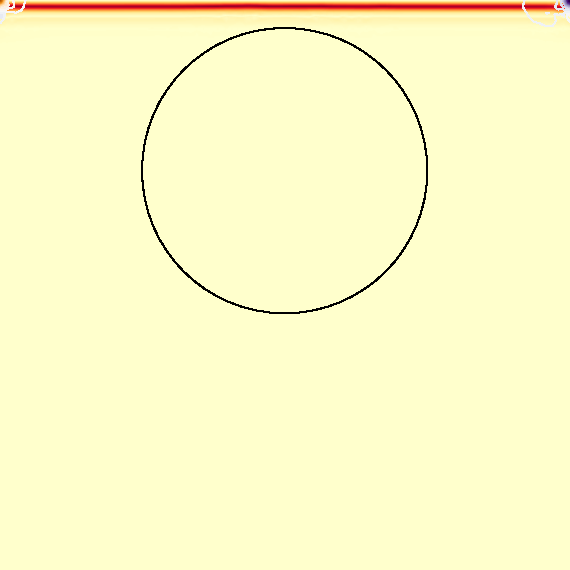
\includegraphics[angle=180,origin=c,height=\IH,keepaspectratio]{images/pu1.pdf}};
  \node[rectangle,anchor=south,draw=black,inner sep=0pt,thick] at (axis cs:0.115,\YA)
    {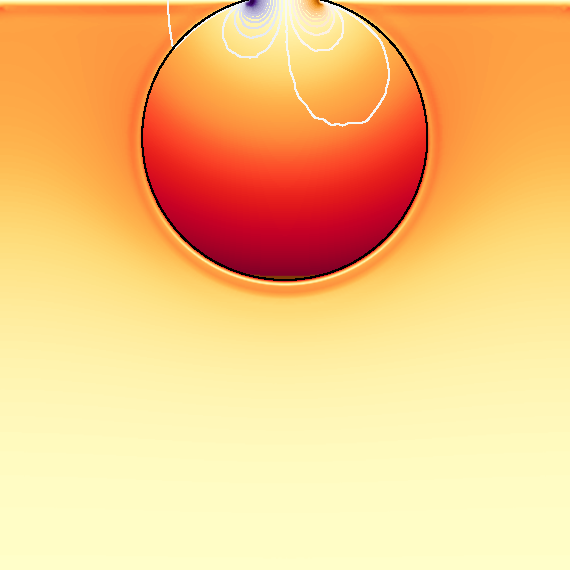
\includegraphics[angle=180,origin=c,height=\IH,keepaspectratio]{images/pu3.pdf}};
  \node[rectangle,anchor=south,draw=black,inner sep=0pt,thick] at (axis cs:0.25,\YA)
    {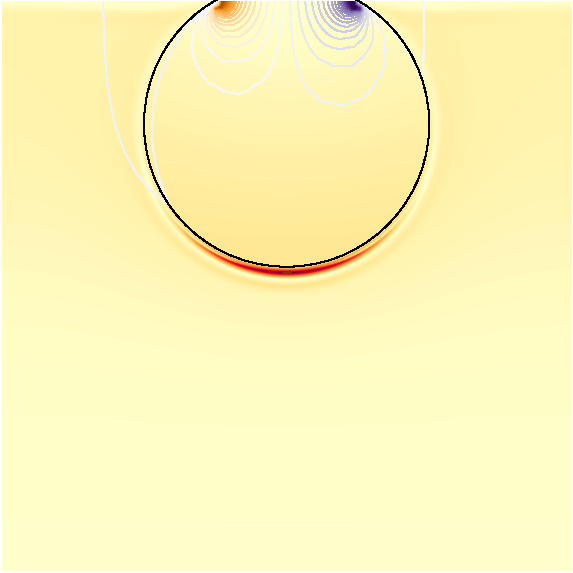
\includegraphics[angle=180,origin=c,height=\IH,keepaspectratio]{images/pu6.pdf}};

  \node[rectangle,anchor=south,draw=black,inner sep=0pt,thick] at (axis cs:0.33,\YA)
    {
\includegraphics[height={\IH-5pt},width=5px]{images/bar1.png}};
  \node[anchor=south,yshift=34pt] at (axis cs:0.33,\YA){\tiny$P$};

  \node[rectangle,anchor=south,draw=black,inner sep=0pt,thick] at (axis cs:0.35,\YA)
    {
\includegraphics[height={\IH-5pt},width=5px]{images/bar2.png}};
  \node[anchor=south,yshift=34pt] at (axis cs:0.35,\YA){\tiny $V$};

  \node[anchor=south,yshift=26pt,xshift=-13pt] at (axis cs:-0.02,\YA){\footnotesize (a)};
  \node[anchor=south,yshift=26pt,xshift=-13pt] at (axis cs:0.115,\YA){\footnotesize (b)};
  \node[anchor=south,yshift=26pt,xshift=-13pt] at (axis cs:0.25,\YA){\footnotesize (c)};
  \node[anchor=south,yshift=26pt,xshift=-13pt] at (axis cs:0.41,0.35){\footnotesize (d)};

  \node [draw,fill=white,anchor=south west] at (rel axis cs: 0.01,{0.01*1.25}) {\shortstack[l]{
    \raisebox{-1.5pt}{\ref{p1}} \tiny $\Delta\!f/N_\mathrm{L}$, sim\\
    \raisebox{-1.5pt}{\ref{p2}} \tiny $\Delta\Gamma/N_\mathrm{L}$, sim }};

    \node [draw,fill=white,anchor=south east] at (rel axis cs: 0.99,{0.01*1.25}) {\shortstack[l]{
    \raisebox{-1.5pt}{\ref{p3}} \tiny $\Delta\!f/N_\mathrm{L}$, theory\\
    \raisebox{-1.5pt}{\ref{p4}} \tiny $\Delta\Gamma/N_\mathrm{L}$, theory}};

  %\node[anchor=south west,xshift=25pt] at (yticklabel cs:0){\includegraphics{lowerspherea.pdf}};
  %\node[anchor=south west,xshift=150pt] at (yticklabel cs:0){\includegraphics{lowersphereb.pdf}};

  \node[anchor=south,scale=1] at (axis cs:0.30,0) {
\definecolor{c5d5d5d}{RGB}{93,93,93}
\begin{tikzpicture}[y=0.80pt, x=0.8pt,yscale=-1, inner sep=0pt, outer sep=0pt]
% path5369
\path[draw=black,line width=0.279pt]
  (27.9622,4.8057)arc(0.000:180.000:3.487)arc(-180.000:0.000:3.487) -- cycle;

% path5369-3
\path[draw=black,miter limit=4.00,line width=0.279pt]
  (30.3336,35.5137)arc(0.000:180.000:5.894)arc(-180.000:0.000:5.894) -- cycle;

\begin{scope}[cm={{0.34868,0.0,0.0,0.34868,(-39.3301,-8.38571)}}]% g5820
  % path5549
  \path[draw=black,line join=round,line cap=round,miter limit=4.00,line
    width=0.279pt] (182.9925,160.3622) -- (177.7360,159.2339) --
    (188.2489,156.9775) -- (182.9925,155.8492);

  % path5549-8
  \path[draw=black,line join=round,line cap=rect,miter limit=4.00,line
    width=0.279pt] (182.9925,164.8751) -- (177.7360,163.7469) --
    (188.2489,161.4904) -- (182.9925,160.3622);

  % path5549-8-9
  \path[draw=black,line join=round,line cap=rect,miter limit=4.00,line
    width=0.279pt] (182.9925,169.3881) -- (177.7360,168.2598) --
    (188.2489,166.0034) -- (182.9925,164.8751);

  % path5549-8-9-4
  \path[draw=black,line join=round,line cap=round,miter limit=4.00,line
    width=0.279pt] (182.9925,173.9010) -- (177.7360,172.7728) --
    (188.2489,170.5163) -- (182.9925,169.3881);

\end{scope}
\begin{scope}[cm={{0.34868,0.0,0.0,0.34868,(-39.3301,-6.29364)}}]% g5725
  % path5549-8-5
  \path[draw=black,line join=round,line cap=butt,miter limit=4.00,line
    width=0.279pt] (197.6282,68.0450) -- (192.3718,66.9168) -- (202.8847,64.6603)
    -- (197.6282,63.5321);

  % path5549-8-9-5
  \path[draw=black,line join=round,line cap=rect,miter limit=4.00,line
    width=0.279pt] (197.6282,72.5580) -- (192.3718,71.4298) -- (202.8847,69.1733)
    -- (197.6282,68.0450);

  % path5549-8-9-4-2
  \path[draw=black,line join=round,line cap=rect,miter limit=4.00,line
    width=0.279pt] (197.6282,77.0709) -- (192.3718,75.9427) -- (202.8847,73.6862)
    -- (197.6282,72.5580);

\end{scope}
\begin{scope}[cm={{0.34868,0.0,0.0,0.34868,(-33.19391,-2.47933)}}]% g5692
  % path5668
  \path[draw=black,line join=miter,line cap=butt,miter limit=4.00,line
    width=0.279pt] (142.5984,55.8015) -- (142.5984,61.4228) -- (157.4016,61.4228)
    -- (157.4016,55.8015);

  % path5670
  \path[draw=black,line join=miter,line cap=butt,line width=0.279pt]
    (150.0000,52.3622) -- (150.0000,57.3622);

  % path5672
  \path[draw=black,line join=miter,line cap=butt,line width=0.279pt]
    (145.0000,57.3622) -- (155.0000,57.3622);

  % path5670-7
  \path[draw=black,line join=miter,line cap=butt,line width=0.279pt]
    (150.0000,61.3622) -- (150.0000,66.3622);

\end{scope}
% path5711
\path[draw=black,line join=round,line cap=round,miter limit=4.00,line
  width=0.279pt] (29.6167,15.8652) -- (29.6167,13.6192);

% path5732
\path[draw=black,line join=miter,line cap=rect,miter limit=4.00,line
  width=0.279pt] (19.1079,15.7782) -- (19.1079,13.6192);

% path5734
\path[draw=black,line join=miter,line cap=rect,miter limit=4.00,line
  width=0.282pt] (29.6129,13.6192) -- (19.3380,13.6192);

% path5736
\path[draw=black,line join=miter,line cap=rect,miter limit=4.00,line
  width=0.279pt] (24.4754,13.3036) .. controls (24.4754,8.6412) and
  (24.4754,8.6412) .. (24.4754,8.6412);

% path5711-2
\path[draw=black,line join=round,line cap=round,miter limit=4.00,line
  width=0.279pt] (29.5786,20.5793) -- (29.5786,22.8254);

% path5732-1
\path[draw=black,line join=miter,line cap=rect,miter limit=4.00,line
  width=0.279pt] (19.1079,20.6597) -- (19.1079,22.8188);

% path5734-9
\path[draw=black,line join=miter,line cap=rect,miter limit=4.00,line
  width=0.282pt] (19.1275,22.8235) -- (29.4024,22.8235);

% path5736-4
\path[draw=black,line join=miter,line cap=rect,miter limit=4.00,line
  width=0.279pt] (24.5125,29.2869) .. controls (24.5125,22.7920) and
  (24.5125,22.7920) .. (24.5125,22.7920);

% path5736-4-0
\path[draw=black,line join=miter,line cap=round,miter limit=4.00,line
  width=0.279pt] (24.4754,45.9556) .. controls (24.4754,41.6169) and
  (24.4754,41.6169) .. (24.4754,41.6169);

% path5736-4-0-1
\path[draw=black,line join=miter,line cap=round,miter limit=4.00,line
  width=0.279pt] (24.4754,56.5885) .. controls (24.4754,52.2498) and
  (24.4754,52.2498) .. (24.4754,52.2498);

% rect3086
\path[fill=c5d5d5d,nonzero rule,rounded corners=0.0000cm] (0.0000,56.4547)
  rectangle (49.0250,60.5717);

% rect3086-6
\path[fill=c5d5d5d,fill opacity=0.399,nonzero rule,rounded corners=0.0000cm]
  (0.0000,26.8859) rectangle (49.0250,56.4547);

% text3138

% text3138-7
\draw [decorate,decoration={brace,mirror}] (0,0) -- (0,26.8859) node [midway,left,xshift=-5pt] {\tiny load};
\draw [decorate,decoration={brace,mirror}] (0,26.8859) -- (0,60.5717) node [midway,left,xshift=-5pt] {\tiny QCM};

% text3142
\path[fill=black] (29.212894,5.8104634) node[right] (text3142) {\tiny $m_\mathrm{L}$};

% text3166
\path[fill=black] (33.049664,19.223736) node[right] (text3166) {\tiny $k_\mathrm{L}$};

% text3316
\path[fill=black] (16.128359,19.223736) node[left] (text3316) {\tiny $\xi_\mathrm{L}$};

% text3138-2
\path[fill=black] (31.584267,36.51849) node[right] (text3138-2) {\tiny $m_\mathrm{q}$};

% text3138-8
\path[fill=black] (27.643841,50.268837) node[right] (text3138-8) {\tiny $k_\mathrm{q}$};
\end{tikzpicture}
};

 \end{axis}
\end{tikzpicture}



\end{document}
